\documentclass[12pt]{article}

\usepackage[a4paper,margin=2.5cm]{geometry}
\usepackage{amsmath, amssymb, amsthm}
\usepackage{bm}
\usepackage{hyperref}
\usepackage{graphicx}
\usepackage{caption}
\usepackage{listings}
\usepackage{xcolor}
\usepackage{float}
\usepackage{placeins}
\graphicspath{{figures/}}

\lstdefinestyle{code}{
  basicstyle=\ttfamily\small,
  numbers=left,
  numberstyle=\tiny,
  numbersep=8pt,
  keywordstyle=\color{blue},
  commentstyle=\color{teal!70!black},
  stringstyle=\color{orange!70!black},
  showstringspaces=false,
  breaklines=true,
  frame=single,
  framerule=0.3pt,
  rulecolor=\color{black!15}
}
\lstset{style=code}

\title{Asynchronous Advantage Actor-Critic (A3C) Tutorial}
\author{}
\date{\today}

\begin{document}
\maketitle

\section{Introduction}
Asynchronous Advantage Actor-Critic (A3C) runs multiple agents in parallel, each updating a shared policy and value network. By decoupling workers and using asynchronous updates, A3C decorrelates experience, stabilizes learning without replay buffers, and exploits multi-core CPU hardware.

\section{Theory and Formulas}
\subsection{Multi-worker Objective}
Each worker maintains local parameters \((\theta', w')\) initialized from global parameters \((\theta, w)\). After collecting a rollout of length \(n\), the worker computes multi-step advantages:
\begin{equation}
A_t = \sum_{k=0}^{n-1} \gamma^k r_{t+k+1} + \gamma^n V_w(s_{t+n}) - V_w(s_t).
\end{equation}
Gradients are accumulated locally before being applied to the shared parameters.

\subsection{Asynchronous Updates}
Policy and value gradients for each worker are
\begin{align}
\nabla_\theta J &\approx \sum_{t} \nabla_\theta \log \pi_\theta(a_t\mid s_t)\, A_t + \beta \nabla_\theta H\big[\pi_\theta(\cdot\mid s_t)\big],\\
\nabla_w L_V &\approx \sum_{t} \partial_w \frac{1}{2} A_t^2,
\end{align}
where \(\beta\) controls entropy regularization. After computing gradients, the worker atomically updates global parameters and syncs local copies.

\subsection{Stability Considerations}
Asynchronous execution increases gradient noise but improves exploration. Using smaller rollout lengths \(n\), gradient clipping, and synchronized learning rates across workers maintains stability. Optimizers such as RMSprop with shared statistics are commonly used.

\section{Applications and Tips}
\begin{itemize}
  \item \textbf{CPU-friendly training}: leverage multi-core servers without large replay buffers.
  \item \textbf{Sparse rewards}: parallel workers discover different trajectories, increasing successful rollouts.
  \item \textbf{Continuous and discrete control}: extend A3C with Gaussian actors or shared convolutional encoders.
  \item \textbf{Best practices}: synchronize parameters periodically, use per-worker learning rate annealing, and monitor gradient norms to detect divergence.
\end{itemize}

\section{Python Practice}
The script \texttt{gen\_a3c\_figures.py} emulates three asynchronous workers solving a cliff-world task. Each worker gathers short rollouts, computes multi-step advantages, and applies gradients to shared actor-critic tables. The script records the aggregated return curve and final policy probabilities.
\begin{lstlisting}[language=Python,caption={Excerpt from gen_a3c_figures.py}]
for worker in range(num_workers):
    states, actions, rewards = collect_rollout(theta_local[worker], V_local[worker])
    advantages = compute_n_step_advantages(states, rewards, V_global)
    grad_theta, grad_V = accumulate_gradients(states, actions, advantages)
    theta_global += actor_lr * grad_theta
    V_global += critic_lr * grad_V
\end{lstlisting}

\section{Result}
\begin{figure}[H]
  \centering
  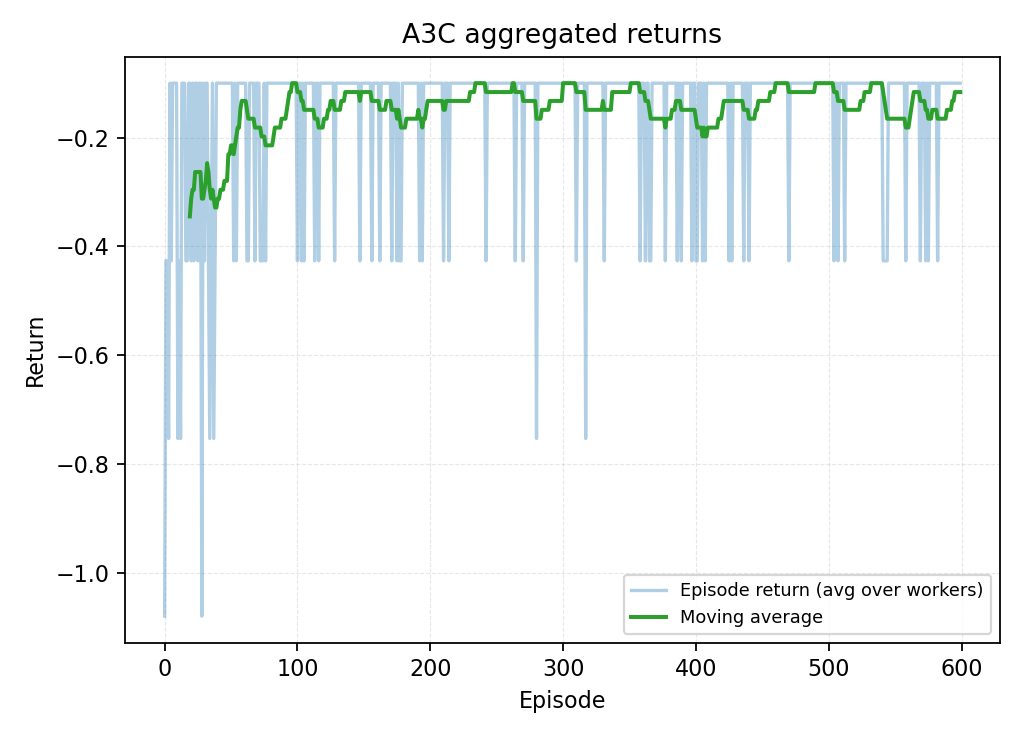
\includegraphics[width=0.8\linewidth]{a3c_returns.png}
  \caption{A3C episode returns aggregated across asynchronous workers}
  \label{fig:a3c_returns}
\end{figure}

\begin{figure}[H]
  \centering
  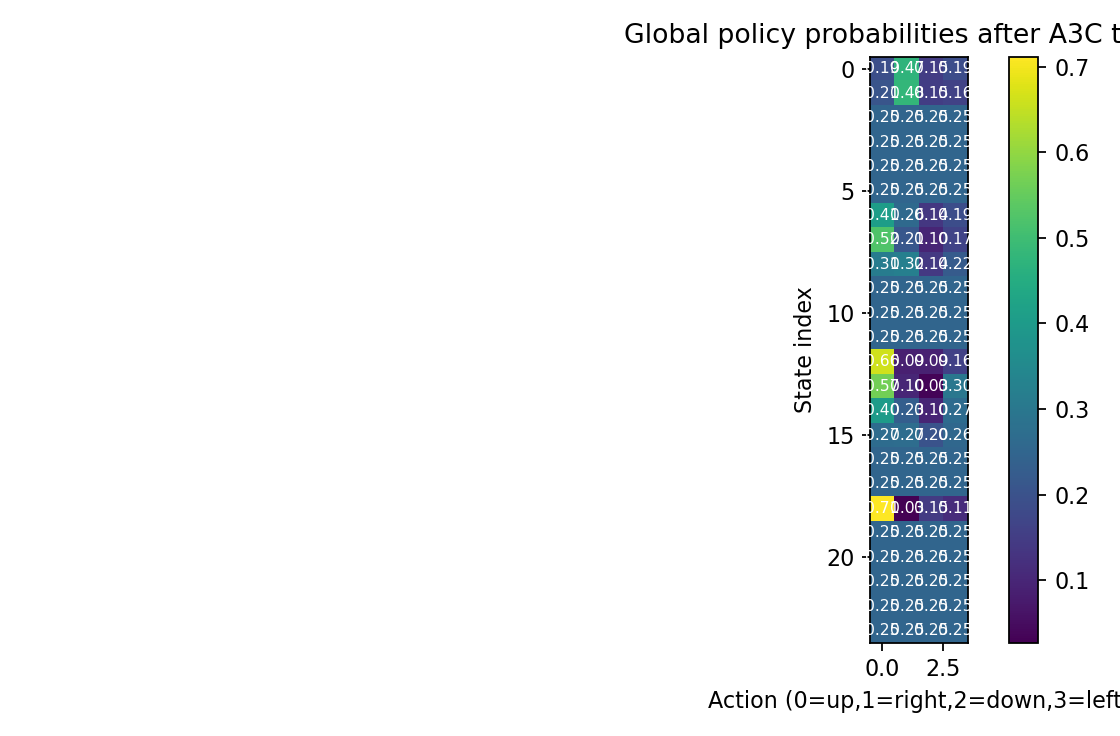
\includegraphics[width=0.82\linewidth]{a3c_policy_heatmap.png}
  \caption{Action probability heatmap of the global policy after training}
  \label{fig:a3c_policy_heatmap}
\end{figure}

\FloatBarrier
\section{Summary}
A3C combines multi-step advantage estimation with asynchronous workers to stabilize on-policy learning without replay buffers. Proper tuning of rollout length, entropy bonuses, and optimizer settings balances gradient noise and convergence speed. The cliff-world example illustrates how worker diversity accelerates policy improvement and yields interpretable action probabilities.

\end{document}